\subsection{Messung bis 1 bar}
In der folgenden Abbildung (\ref{fig:aufbau1}) ist der Aufbau für die 1 bar Messung
zu sehen.

\begin{figure}
  \centering
  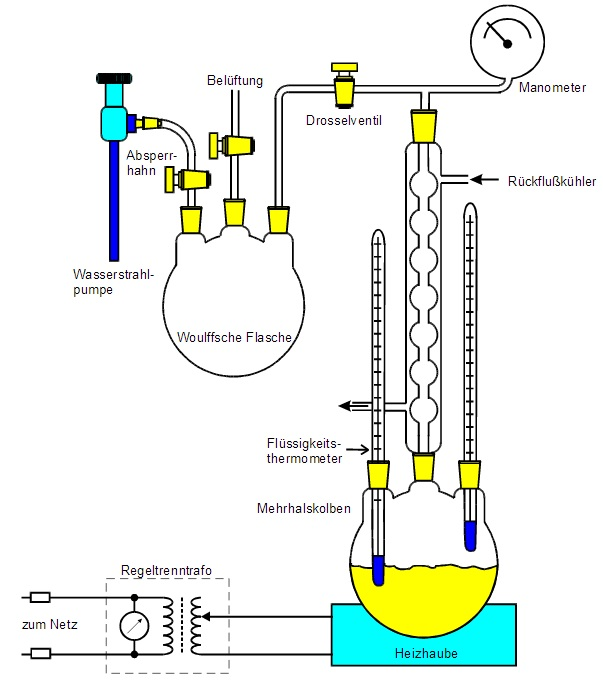
\includegraphics[height=10cm]{Aufbau1.jpg}
  \caption{Messapparatur für $p ≤ 1 bar$}
  \label{fig:aufbau1}
\end{figure}

Zu Beginn wird das System mit einer Wasserstrahlpumpe evakuiert, dazu müssen der
Absperrhahn und das Drosselventil geöffnet und das Belüftungsventil geschlossen sein.
Sobald der Druck nicht weiter sinkt, schließt man das Drosselventil und den
Absperrhahn und stellt die Wasserstrahlpumpe wieder aus. Nun wird die Wasserkühlung
angestellt, um aufsteigende Dämpfe zu unterdrücken. Dann wird die Heizhaube angestellt,
um das Wasser zu erhitzen. Während des Erhitzens muss die Kühlung ständig neu
reguliert werden, damit sie weder zu stark, noch zu schwach wirkt.
Sobald das Wasser nun siedet, liest man die Temperatur, im Gasraum,
mit dem dazugehörigen Druck, am Manometer, in festen Abständen ab.
Wenn ein Druck von 1 bar erreicht wurde ist die Messung beendet.

\subsection{Messung bis 15 bar}
In der nächsten Abbildung (\ref{fig:aufbau2}) ist der Aufbau für die 15 bar Messung
zu sehen.

\begin{figure}
  \centering
  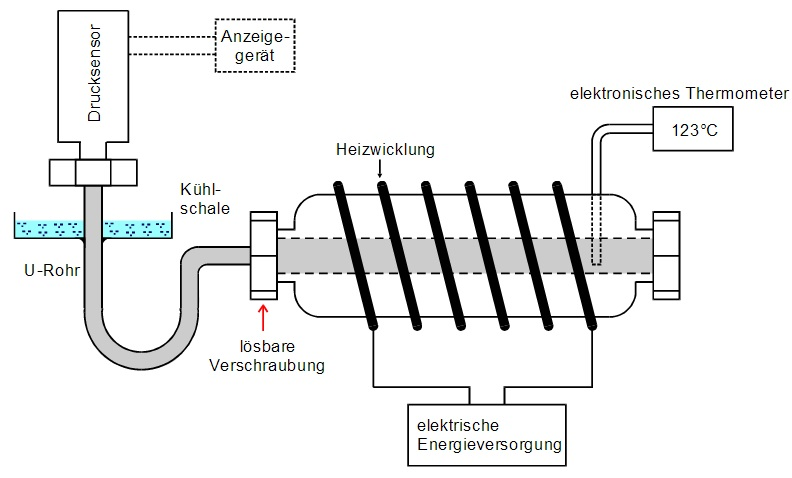
\includegraphics[height=10cm]{Aufbau2.jpg}
  \caption{Messapparatur für $p ≤ 15 bar$}
  \label{fig:aufbau2}
\end{figure}

Die Apparatur ist bereits mit Wasser befüllt. Um die Messung zu starten müssen
lediglich die Heizwicklung und der Drucksensor angeschaltet werden. Auch bei
dieser Messung werden gleichzeitg die Temperatur und der Druck in regelmäßgen
Abständen abgelesen, diesmal bis ein Druck von 15 bar erreicht wird.
